\documentclass{article}
\usepackage[utf8]{inputenc}
\usepackage{listings}
\usepackage{todonotes}
\usepackage{amsmath}

\title{EMBS Autumn Assessment}
\author{Y6385133}
\date{Autumn 2012}

\begin{document}

\maketitle

\section{Modelling}
I chose to model the solution using Mote Runner SDK. The main reasons against using another solution were:

\begin{description}
    \item[Differences in implementation details] \hfill \\
        There is no guarantee that applications such as ptollemy would exhibit the same characteristics as a mote
    \item[Time constraints] \hfill \\
        I expected the majority of my time would be taken up with debugging the mote {SDK}
\end{description}

\section{Implementation}

My original implementation observed a channel until it had determined the period, and then analysed
the next sink. This worked, but in the worst case situation where the $Sink_A$ has $n=1500$ and $t=10$ the source could block
for ~ 35s -- over half the time of the entire simulation -- before it analyses other sinks. See figure \ref{fig:long-blocking}.


\begin{figure}[h]
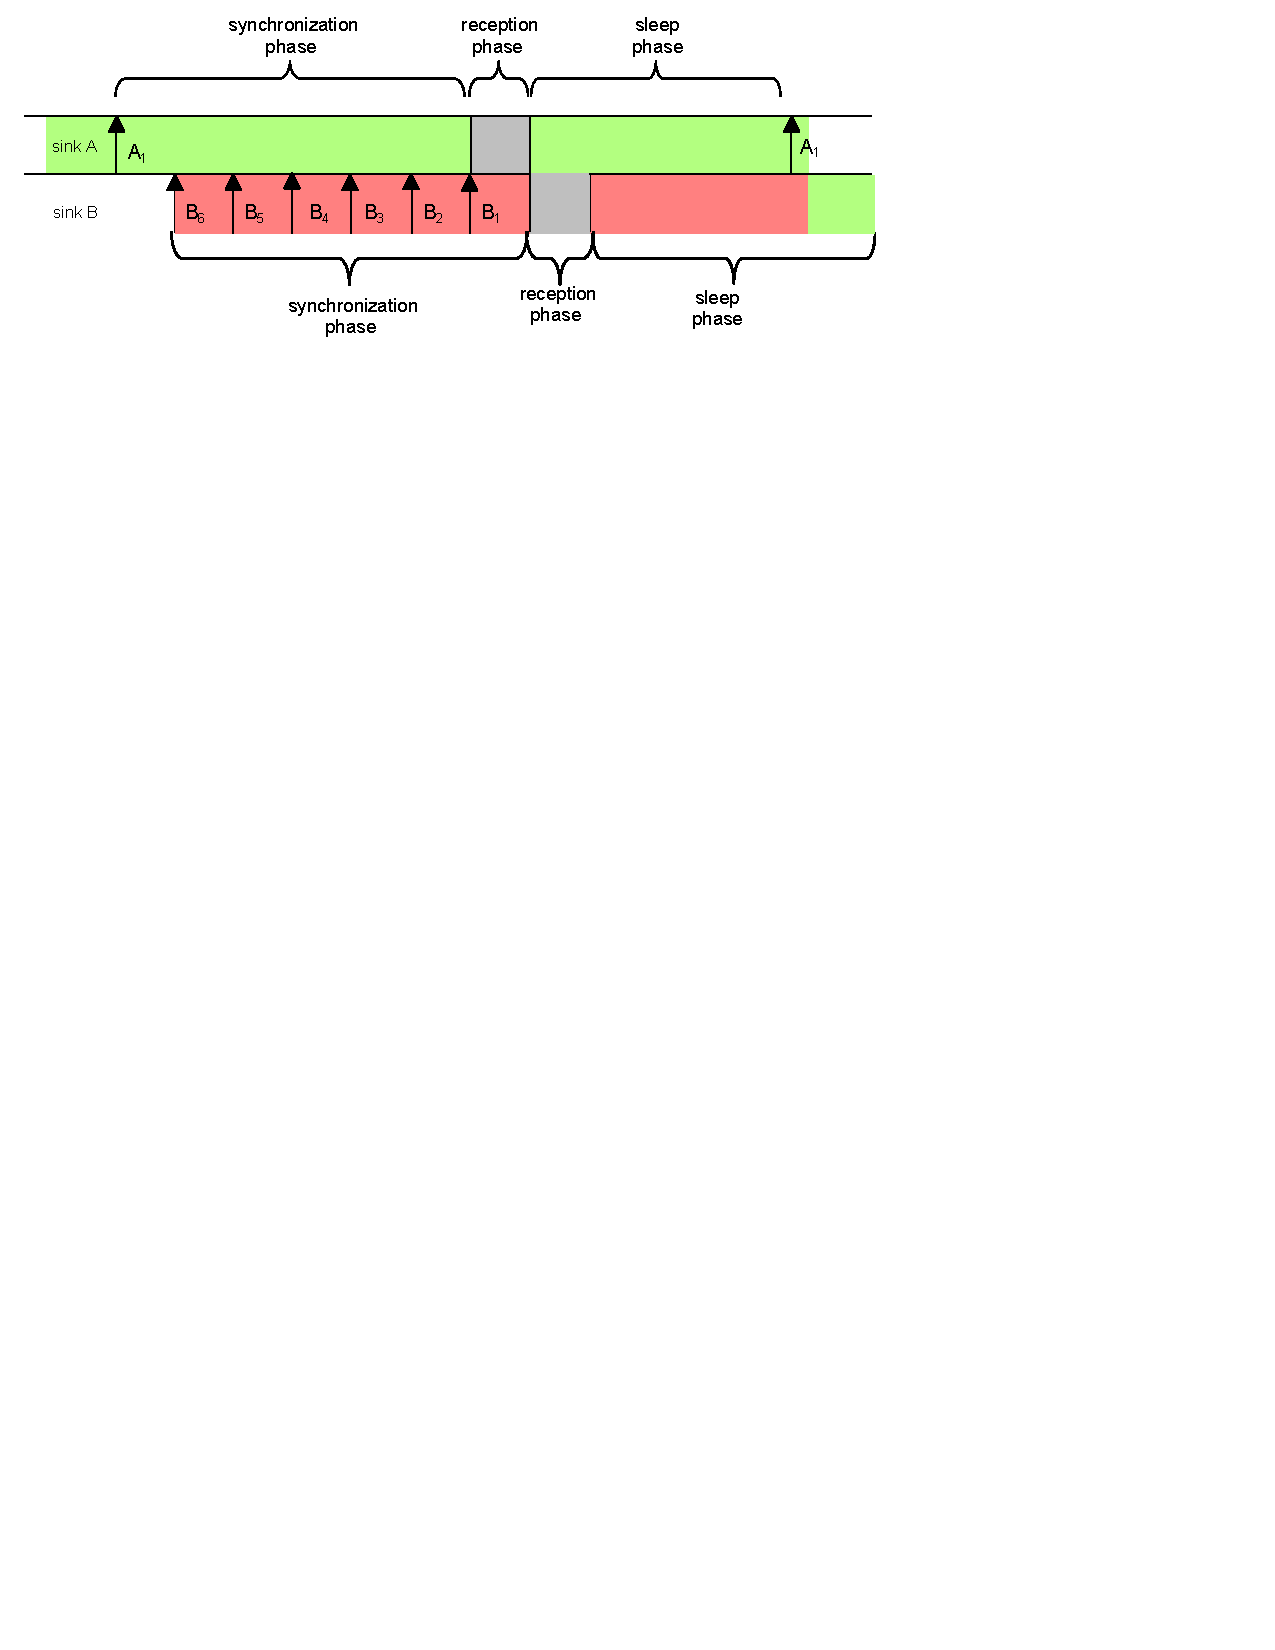
\includegraphics[trim=1cm 22cm 1cm 1cm]{embs-blocking}
\caption{Without a timeout the source can block for too long and miss other phases}
\label{fig:long-blocking}
\end{figure}

To fix this I added a timeout that restricts the time the source can spend trying to analyse a
channel when there are other periods that need estimating.

The general case for determining a sink's period $t$ involves observing two of the sequence numbers ($n_1, n_2$) emitted by a sink,
recording the times they were observed ($r_1, r_2$) and then calculating:

$$t = \frac{r_2 - r_1} {n_1 - n_2}$$

This allows the period to be calculated without observing consecutive sequence numbers, however the two
sequence numbers must be observed within the same synchronisation phase. In the case where $n=1$ this is impossible,
so I added a special case that calculates

$$t = \frac{r_2 -r_1} {12}$$

However, this can be problematic if the $n_2$ is not in the cycle after $n_1$'s. One countermeasure is to ignore
periods $t > 1600$ (+100ms to allow for clock drift)


When $n_2 > n_1$ we cannot reliably calculate the period as the second
sequence number may not be the sink's $n_max$, thus giving a larger $t$, which could cause us to transmit outside
of the reception period. In this instance $n1$ is replaced with $n_2$'s values and $n_2$ is reset.

\paragraph{}
There is a hard limit of 1600ms to prevent obviously erroneous periods.

\section{Clock Drift}

This is inevitable in systems without a centralised clock, especially when wireless communication is involved.
To help combat drift the source always performs calculations using times events were triggered at, rather than 
`current' time. After each broadcast the source schedules a new broadcast in $t * (11 + n)$ ticks and a resync in 
$(t * (10 + n)) - x$ ticks. The resync is used to verify that the estimated reception period is accurate.
Unfortunately, this is occasionally missed due to competing transmission slots.

\section{Power Saving}

My implementation saves power by scaling down the transmission power based on the signal strength of received packets and turning
off LEDs(when not debugging).
Received power strength is between $0-255$ and transmission power $0-63$. Calculating min power needed to send to $sink_X$:

$$
\mathit{tx\_power}_x = \frac{\mathit{rx\_power}_x} {255} \times 63
$$

However using this exact value will mean a different min power is required as noise/distance from sink changes. 
Instead I transmit at double the minimum required power.

$$
\mathit{tx\_power}_x = max(63, \frac{\mathit{rx\_power}_x} {255} \times 63)
$$

The above operation can be approximated using multiplications of powers of 2, aka bit shifts.

\begin{align*}
\mathit{tx\_power}_x
&= \mathit{rx\_power}_x \times 2^{-8} \times 2^6 \\
&= \mathit{rx\_power}_x \times 2^{-2}
\end{align*}

\section{Verification}

The SDK's netview tool was used to confirm reduction in TX power, however it appears there's a bug
that reports an extreme increase in current when signal strengths other than max are used (figure \ref{fig:crazy-power})

\begin{figure}
\noindent\hspace*{-60pt}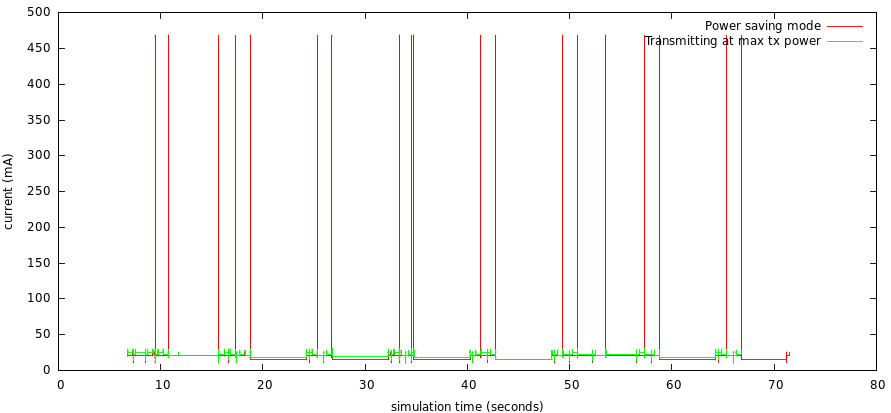
\includegraphics[scale=0.5]{power-consumption.png}
\caption{Bug in power consumption measurements}
\label{fig:crazy-power}
\end{figure}

Ignoring erroneous values yields figure \ref{fig-power-consumption}.

\begin{figure}
  \noindent\hspace*{-60pt}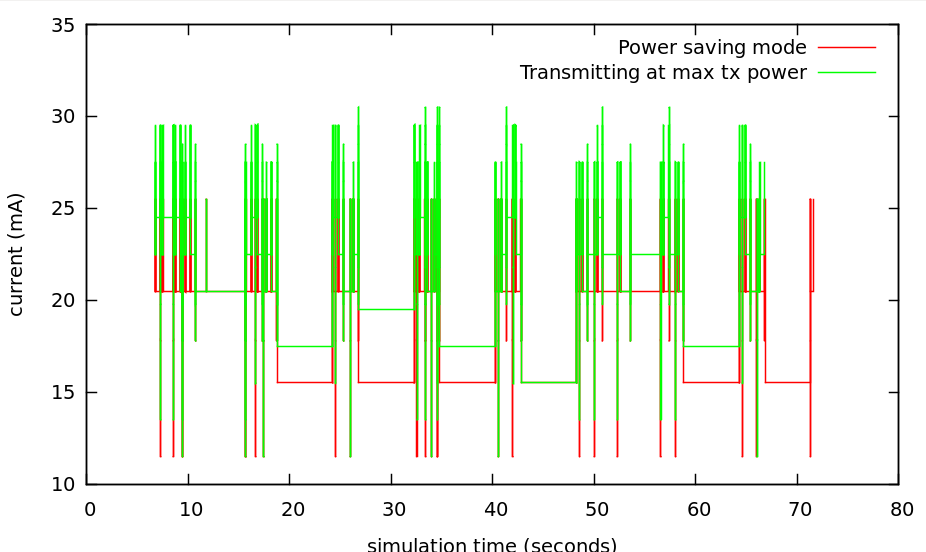
\includegraphics[scale=0.5]{power-consumption-saving.png}
  \caption{Consumption sans bugged values. Note that PSM uses on average less power than max power}
  \label{fig:crazy-power}
\end{figure}


I also used a script by another student (not included) to generate sinks with different parameters,
and automated it to test for multiple scenarios:

\begin{figure}
\begin{tabular}{|c|c|c|c||c|c|c|c||c|c|c|c|}
  \hline 
  \multicolumn{4}{|c||}{$Sink_{A}$} & \multicolumn{4}{c||}{$Sink_{B}$} & \multicolumn{4}{c|}{$Sink_{C}$}\tabularnewline
  \hline 
  $n$ & $t$(ms) & $A$ & $R$ & $n$ & $t$(ms) & $A$ & $R$ & $n$ & $t$(ms) & $A$ & $R$\tabularnewline
  \hline 
  \hline 
  10 & 500 & 6 & 0 & 4 & 700 & 6 & 0 & 5 & 1500 & 3 & 0\tabularnewline
  \hline 
  2 & 541 & 9 & 0 & 3 & 912 & 5 & 0 & 6 & 1101 & 3 & 0\tabularnewline
  \hline 
  6 & 1407 & 3 & 0 & 5 & 567 & 7 & 0 & 2 & 1207 & 3 & 0\tabularnewline
  \hline 
  2 & 725 & 7 & 0 & 8 & 868 & 4 & 0 & 4 & 1043 & 4 & 0\tabularnewline
  \hline 
  10 & 683 & 4 & 0 & 7 & 1308 & 3 & 0 & 2 & 685 & 6 & 0\tabularnewline
  \hline 
  1 & 683 & 7 & 0 & 7 & 1308 & 3 & 0 & 2 & 685 & 6 & 0\tabularnewline
  \hline 
  2 & 500 & 9 & 0 & 2 & 500 & 9 & 0 & 2 & 500 & 9 & 0\tabularnewline
  \hline 
  7 & 1308 & 3 & 0 & 1 & 1500 & 1 & 0 & 2 & 685 & 5 & 0\tabularnewline
  \hline 
  8 & 1500 & 2 & 0 & 1 & 1000 & 0 & 0 & 7 & 1000 & 3 & 0\tabularnewline
  \hline 
\end{tabular}
\caption{$A$: packets sent in RX period, $R$: packets sent outside RX period}
\end{figure}
\paragraph{}

These values were all observed in the simulator so performance on hardware may be different.\

\paragraph{}

\lstinputlisting[language=bash,numbers=left,frame=single]{../benchmark.sh}
\end{document}

